\section{Wprowadzenie}
\label{sec:wprowadzenie}

We współczesnym świecie, pełnym pospiechu, zabiegania i~nowinek technologicznych, internet stanowi nieodzowna część naszego życia --- jest wręcz nieodłącznym jego elementem. Jednakże czymże byłby internet, bez możliwości kontaktowania się z~przyjaciółmi, zdobywania informacji o~wydarzeniach kulturalnych czy rozrywkowych. W tym celu powstały media społecznościowe, ale czy aby na pewno? Jeszcze do niedawna taki osąd dotyczący mediów społecznościowych funkcjonował. Uważano iż to kolejne po komunikatorach narzędzie do komunikacji pomiędzy młodymi ludźmi. Zanim jednak przejdziemy do meritum naszej pracy i~opowiemy o~tym jakie możliwości dają nam media społecznościowe, wyjaśnijmy czym one w ogóle są.

\subsection{Definicja mediów społecznościowych}

\begin{defn}[Media społecznościowe, z~j. ang.social media] określenie odnosi się do ogólnie pojętego korzystania z~internetowych i~mobilnych technologii, by przekształcić komunikację w interaktywny dialog.
\end{defn}

Andreas Kaplan i~Michael Haenlein definiują media społecznościowe jako ,,grupę bazujących na internetowych rozwiązaniach aplikacji, które opierają się na ideologicznych i~technologicznych podstawach Web 2.0, i~które to umożliwiają tworzenie i~wymianę wygenerowanych przez użytkowników treści'' \cite{url:wiki-media-spolecznosciowe}. Media społecznościowe to media do społecznościowych interakcji w postaci rozbudowanego zestawu narzędzi komunikacyjnych wykraczających poza dotychczasową komunikację społecznościową. Dzięki wszechobecnej dostępności i~skalowalności technik komunikacyjnych, media społecznościowe diametralnie zmieniły sposób komunikacji zarówno organizacji, społeczności, jak i~indywidualnych użytkowników \cite{url:wiki-media-spolecznosciowe}.

%--------------------------------------

\subsection{Rodzaje mediów społecznościowych}
Social media odznaczają się dużą interaktywnością, sfokusowane są zarówno na kreowanie sieci kontaktów, jak również relacji. Umożliwiają dzielenie się materiałami audio, wideo i~zdjęciami. Dzięki tym rozwiązaniom możliwa jest wielokierunkowa wymiana wszystkich materiałów, które użytkownicy udostępniają na swoich kontach-profilach. Użytkownicy tych mediów skupiają się także w podgrupy wg. zainteresowań, poglądów, bądź też społeczności lokalnej, lub tak jak nasza grupa wg kierunku studiów \cite{url:kursusability-social-media}. 

Media społecznościowe dla firm stanowią nieocenione źródło tworzonych za sprawą użytkowników treści, które noszą nazwę UGC (ang. \textit{User-generated content}) lub CGM (ang. \textit{Consumer Generated Media}) \cite{url:wiki-mashup}.

%-------------------------------------------------------------------------

\subsection{Podział mediów społecznościowych}

\begin{figure}[!h]
\centering
    \scalebox{0.9}
    {
        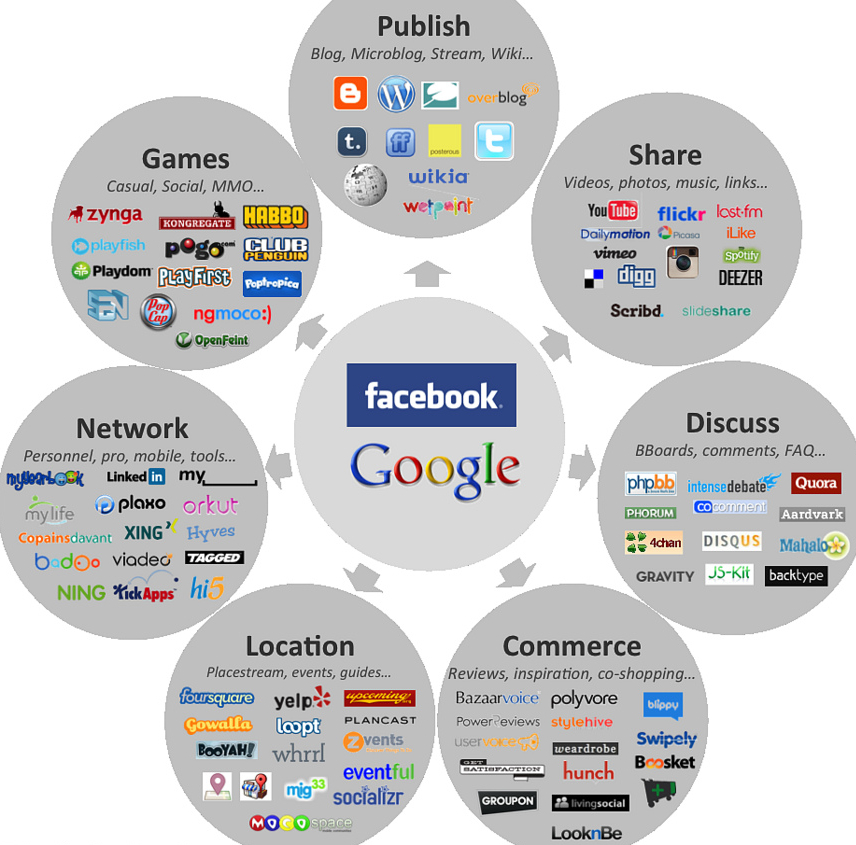
\includegraphics{images/lukasz/social-media-landscape-20111_k.jpg}
    }
    \captionsource{Podział mediów społecznościowych}{\url{http://jonathanwichmann.files.wordpress.com/2011/08/social-media-landscape-20111_k.jpg}}
    \label{fig:sample-google-plus-company-profile-page}
\end{figure}

Powyższy schemat przedstawia czym faktycznie są media społecznościowe, jakie mają funkcjonalności, i~co umożliwiają osobom, które z~nich korzystają, czyli nam użytkownikom. Do tych możliwości zaliczyć można: narzędzia umożliwiające rozmowę online, serwisy zaprojektowane do dzielenia się treścią, umożliwiające publikowanie oraz wspólne tworzenie treści oraz publikujące informację naukowe, gry online, społecznościowe światy wirtualne, serwisy blogowe, a~także tworzenie materiałów wideo na urządzenia mobilne w tym telefony komórkowe.

\subsubsection{Rodzaje mediów społecznościowych}

Powyższy rysunek dzieli nam media społecznościowe w sposób umowny. Poniżej przedstawimy te rodzaje social media, które są w Polsce najpopularniejsze.\\

\noindent Są to:

\begin{itemize}
\item Serwisy społecznościowe
\item Blogi
\item Mikroblogi
\item Wiki
\end{itemize}

W naszym opracowaniu skupimy się wyłącznie na serwisach społecznościowych, które zostaną omówione szerzej.

\subsection{Serwisy społecznościowe}

Serwisy społecznościowe są w tej chwili najbardziej dynamicznie rozwijanym się medium społecznościowym w obszarze języka polskiego. Nazywany jest także sieciami społecznymi lub też social networking. Charakteryzują się tym, iż przy ich pomocy jest utrzymywana, jak również zawierana znajomość pomiędzy użytkownikami. W książce pt. ,,Nowy marketing'' jej autor Dominik Kaznowski, serwisy społecznościowe przedstawia w taki oto sposób ,,Jedną z~najważniejszych cech jest właśnie duża interaktywność nastawiona na kreowanie sieci kontaktów i~relacji. Najczęściej przybiera to formę listy znajomych, z~którymi internauci wchodzą w mniejszą lub większą interakcję'' \cite{url:kursusability-social-media}.\\

\noindent Obecnie serwisy społecznościowe wyposażone są w takie funkcje jak:

\begin{itemize}
\item Profile użytkowników --- pełnią funkcję wizytówki, strony prywatnej użytkownika, na której znajdują się podstawowe informacje o~nim, jego zdjęcia, pliki audio i~video, lista ulubionych stron, grupy dyskusyjne, do których należy, lista znajomych i~tablica, na której znajdują się informacje o~aktywnościach użytkownika i~jego wpisy;

\item Listy kontaktów --- listy profili osób, z~którymi użytkownik utrzymuje kontakty tzw. znajomi; możliwość zapraszania;

\item Fora dyskusyjne --- skupione wokół danego tematu, organizacji lub działalności grupy, na których większa liczba osób może wymieniać poglądy, wypowiadać się, publikować zdjęcia itp.;

\item Fanpage’e --- profile zakładane zazwyczaj przez firmy, organizacje, grupy; posiadają              niedostępną dla użytkowników indywidualnych możliwość posiadania fanów --- osób,              które „lubią” tę stronę, są narzędziem promowania zdarzeń, produktów i~idei;

\item Wewnętrzną pocztę --- możliwość przesyłania wiadomości między użytkownikami serwisu, która nie wymaga zakładania osobnego konta;

\item Wydarzenia;

\item Czaty, komunikatory --- umożliwiające komunikację ze znajomymi w czasie rzeczywistym w ramach jednego serwisu;

\item Funkcjonalności o~charakterze mikroblogowym --- służą do informowania znajomych o~bieżących sprawach w formie krótkich opisów tzw. postów;

\item Współdzielenie plików audio, video, zdjęć oraz linków --- powiązana z~postami możliwość prezentowania znajomym materiałów audio, video, zdjęć oraz linków;
           
\item Wewnętrzne gry, quizy, aplikacje, których tworzenie jest dostępne dla użytkowników,

\item Powiadomienia --- polegają one na tym, że użytkownik serwisu społecznościowego otrzymuje e-maile na podany przez siebie adres z~informacjami o~otrzymanych             zaproszeniach, wydarzeniach czy komentarzach związanych z~profilem użytkownika i~jego znajomymi.
\end{itemize}

%----------------------------------

\subsubsection{Serwisy społecznościowe w Polsce}

\begin{figure}[!h]
\centering
    \scalebox{0.5}
    {
        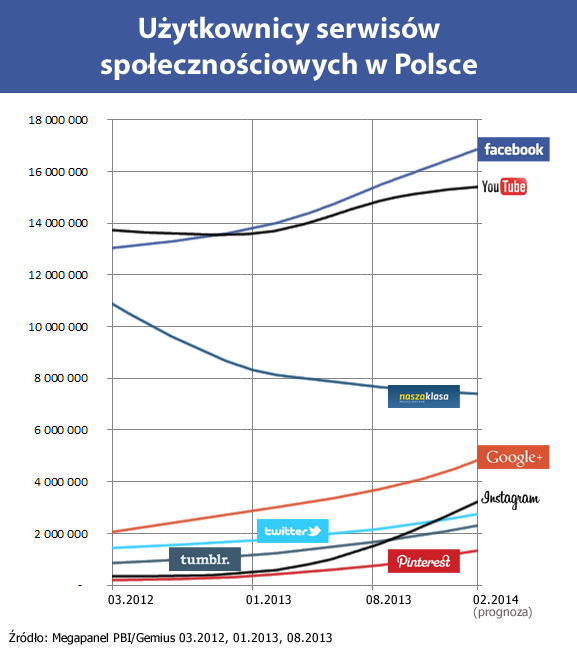
\includegraphics{images/lukasz/analiza.png}
    }
    \captionsource{Ranking mediów społecznościowych w Polsce}{Megapanel PBI/Gemius 03.2012, 01.2013, 08.2013}
    \label{fig:uzytkownicy-mediow-spolecznosciowych-w-polsce}
\end{figure}


Na wykresie z~rysunku \ref{fig:uzytkownicy-mediow-spolecznosciowych-w-polsce} widać, iż najpopularniejszymi serwisami społecznościowymi w naszym kraju jest Facebook --- ok 17 mln użytkowników, następnie, Youtube --- blisko 16 mln użytkowników, następnie nasza klasa --- ok 8 mln użytkowników i~Google+ --- ok 5 mln użytkowników.\\

Nasza praca traktować, będzie o~możliwościach promocji w portalach społecznościowych, a~to jest możliwe de-facto w dwóch serwisach z~wyżej wymienionych --- Facebook oraz Google+ i~to na nich skupiliśmy się w niniejszym opracowaniu.

